\begin{figure*}[tb]
	\centering
	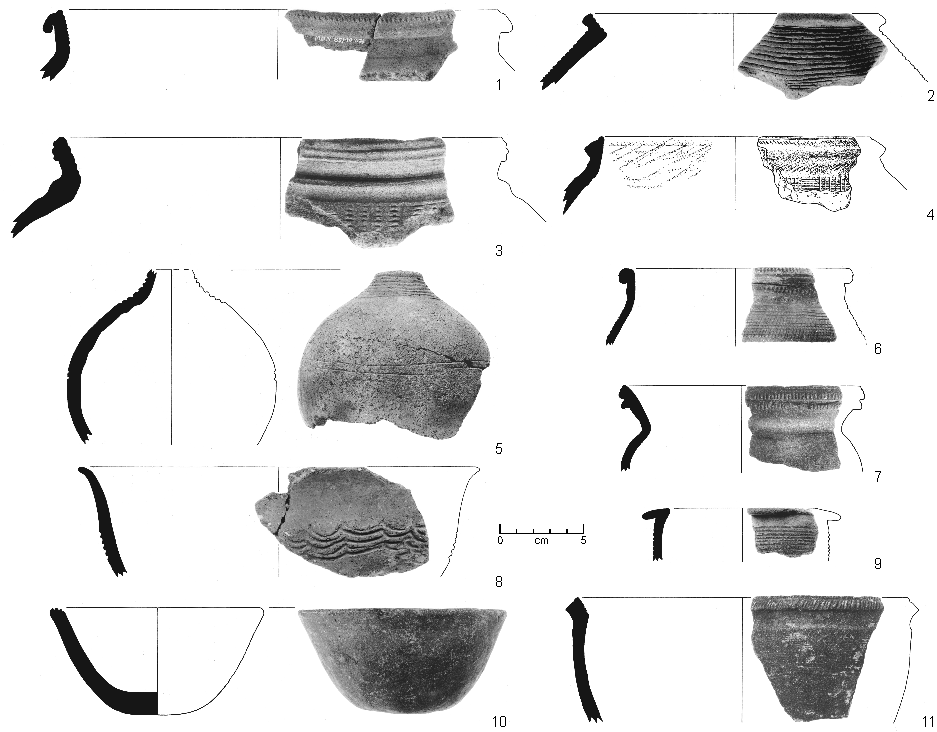
\includegraphics[width=\textwidth]{fig/DON-Typen.pdf}
	\caption{Dongo-Gruppe: Typvertreter.\\1:~Taf.~9.7; 2:~Taf.~8.6; 3:~Taf.~9.8; 4:~Taf.~11.4; 5:~Taf.~7.13; 6:~Taf.~11.3; 7:~Taf.~10.6; 8:~Taf.~8.1; 9:~Taf.~7.14; 10:~Taf.~8.3; 11:~Taf.~10.3.}
	\label{fig:DON_Typverteter}
\end{figure*}

\subsubsection{Dongo-Gruppe}\label{sec:DON-Gr}

Die Dongo-Gruppe beschreibt eine ritzverzierte Keramik, die vor allem entlang des mittleren \mbox{Ubangi} verbreitet ist (Abb.~\ref{fig:DON_Verbreitung}). Bis auf eine potenziell zur Dongo-Gruppe gehörende GE aus einem dem Befund MLB~85/1-3-2 (Kat.-Nr.~2) zuweisbaren Komplex von Surveyfunden\footnote{Es handelt sich um den Komplex MLB~85/104, der sich \enquote{unmittelbar rechts neben MLB 85/1} (Kat.-Nr.~1) befunden hat und unter anderem ein Gefäß der Batalimo-Maluba-Gruppe enthielt (Abb.~\ref{Fig-BatMLB-Typvertreter}.5; Feldbuch \textsc{Eggert} 05.09.1985). In diesem Bereich wurde später die Grube MLB~85/1-3-2 (Kat.-Nr.~2) ausgegraben.} an der am unteren Lua gelegenen Fundstelle Maluba (Fpl.~230) stammt alles dieser Stilgruppe zugewiesene Material aus Oberflächenabsammlungen. Die Beschreibung der Stilgruppe basiert auf insgesamt 111~GE, von denen 67~GE zweifelsfrei der Stilgruppe zugewiesen wurden, sowie 37 ausgezählten Stücken. 

\paragraph{Technologische Merkmale}\hspace{-.5em}|\hspace{.5em}%
Die Keramik der Dongo-Gruppe weist eine starke Heterogenität bezüglich der vertretenen \textit{Fabrics} auf. Die Typen 4a (19\,\%) und 4c (14\,\%) sind am häufigsten vertreten. Mit jeweils über 10\,\% ließen sich die Varianten 7d (12\,\%), 3c (11\,\%), 7c (10\,\%) sowie 8a (10\,\%) beobachten. Diese Verteilung der \textit{Fabrics} spiegelt den grundsätzlich mittleren (36\,\%) bis hohen (33\,\%) Anteil nichtplastischer Partikel im Scherben wider. Es handelt sich größtenteils um heterogene Mischungen von Quarzsanden, die in einigen Fällen auch Anteile von Glimmer und seltener auch Laterit enthalten. Die meisten Stücke zeigen eine glatte oder nur leicht raue Oberfläche, die in einigen Fällen auch leicht sandig ist. Die Färbung der Scherben der Dongo-Gruppe weist auf die Nutzung weiß- (33\,\%) wie auch rotbrennender Tone (26\,\%) hin. Das Gros des Materials (41\,\%) zeigt jedoch eine beige, graue sowie schwarze Färbung, wodurch keine zweifelsfreie Ansprache der Brennfarbe der genutzten Tone möglich ist. Dieser Befund unterstreicht die heterogene Natur der technischen Eigenschaften der Dongo-Keramik. Die Wandungsstärke der Dongo-Keramik liegt im Mittel bei 6,8\,mm mit einer Varianz von 2,3\,mm.

\paragraph{Formen}\hspace{-.5em}|\hspace{.5em}%
Bei insgesamt 84~GE, welche der Dongo-Gruppe zugerechnet wurden, konnte die Gefäßform beschrieben werden. Den überwiegenden Teil (58\,\%) machen flache Gefäße mit geschweifter Wandung und ohne ausgearbeiteten Halsbereich aus (Typ~E; Abb.~\ref{fig:DON_Typverteter}.1--4, 6--7), gefolgt von schalenförmigen Gefäßen mit konvexer Wandung (Typ~I; 24\,\%; Abb.~\ref{fig:DON_Typverteter}.8, 10). Weitere Gefäßformen, wie Flaschen (Typ~A; Abb.~\ref{fig:DON_Typverteter}.5) oder schalenförmige Gefäße mit einbiegendem Rand (Typ~H; Abb.~\ref{fig:DON_Typverteter}.9) sind nur vereinzelt vertreten. Aufgrund der Fragmentierung der größtenteils bei Oberflächensurveys gemachten Funde kann in vielen Fällen eine klare Zuweisung nicht erfolgen. Der Bauchbereich der Dongo-Keramik ist regelmäßig konvex ausgeführt (66\,\%; Abb.~\ref{fig:DON_Typverteter}.5, 7). Seltener lassen sich auch stark (7\,\%) sowie schwach konvexe Wandungen (7\,\%; Abb.~\ref{fig:DON_Typverteter}.8--9) beobachten. Die Ränder der Dongo-Gruppe zeigen ebenfalls eine starke Heterogenität. Bei insgesamt 98~GE können zusammen 19 Randformen unterschieden werden. Die häufigste Randform sind sehr kurze ausbiegende Ränder (B1.1, 22\,\%), die ohne eine Halspartie direkt aus dem Schulterbereich der Gefäße hervorgehen. Ebenfalls charakteristisch sind kurz ausbiegende bis gerade Ränder mit einer im Profil dreieckigen Randleiste (A2.3; 18\,\%). Die Halspartie ist häufig überhaupt nicht (29\,\%) oder nur kurz ausgeführt (27\,\%) und der Schulterbereich der Gefäße ist in der Regel konvex (60\,\%; Abb.~\ref{fig:DON_Typverteter}.5, 7). In geringerem Maße kommen auch gerade Schulterpartieren vor (26\,\%; Abb.~\ref{fig:DON_Typverteter}.2, 6). Der Dongo-Gruppe können gegenwärtig lediglich zwei eindeutige Bodenstücke zugerechnet werden. Während eine GE einen flachen Standboden aufweist (B4), ließ sich an der zweiten GE ein Linsenboden beobachten (B2; Abb.~\ref{fig:DON_Typverteter}.10).


\paragraph{Verzierungen}\hspace{-.5em}|\hspace{.5em}%
Die Verzierungspraxis der Dongo-Keramik wird von horizontalen Ritzlinien dominiert (Tab.~\ref{tab:Verzierungselemente}: 02.1; 67\,\%). Diese finden sich regelhaft an der Innenseite der Ränder (Anlage~4\subref{fig:DON_Verz}; \ref{fig:DON_Typverteter}.1--3). Neben horizontalen Rillen ließen sich nur sehr vereinzelt andere Verzierungselemente feststellen. Unter anderem wurde bei zwei GE vegetabilischer \textit{knotted strip}-Roulette (Tab.~\ref{tab:Verzierungselemente}: 21.1) sowie an einer weiteren, potenziell der Dongo-Gruppe zurechenbaren GE Schnitzroulette (Tab.~\ref{tab:Verzierungselemente}: 21.10; Taf.~21.3) beobachtet. In ebenfalls geringen Anteilen ließen sich \textit{Schachbrettmuster} (Tab.~\ref{tab:Verzierungselemente}: 01.3; 5\,\%; Abb.~\ref{fig:DON_Typverteter}.6) und diagonale (Tab.~\ref{tab:Verzierungselemente}: 04.12; 4\,\%) sowie vertikale Eindrücke (Tab.~\ref{tab:Verzierungselemente}: 04.15; 4\,\%; Abb.~\ref{fig:DON_Typverteter}.1, 4, 6, 7, 11)  identifizieren. Die genannten Eindrücke fanden sich fast ausschließlich an der Randlippe (Anlage~4\subref{fig:DON_Verz}).

\begin{figure*}[p]
	\centering
	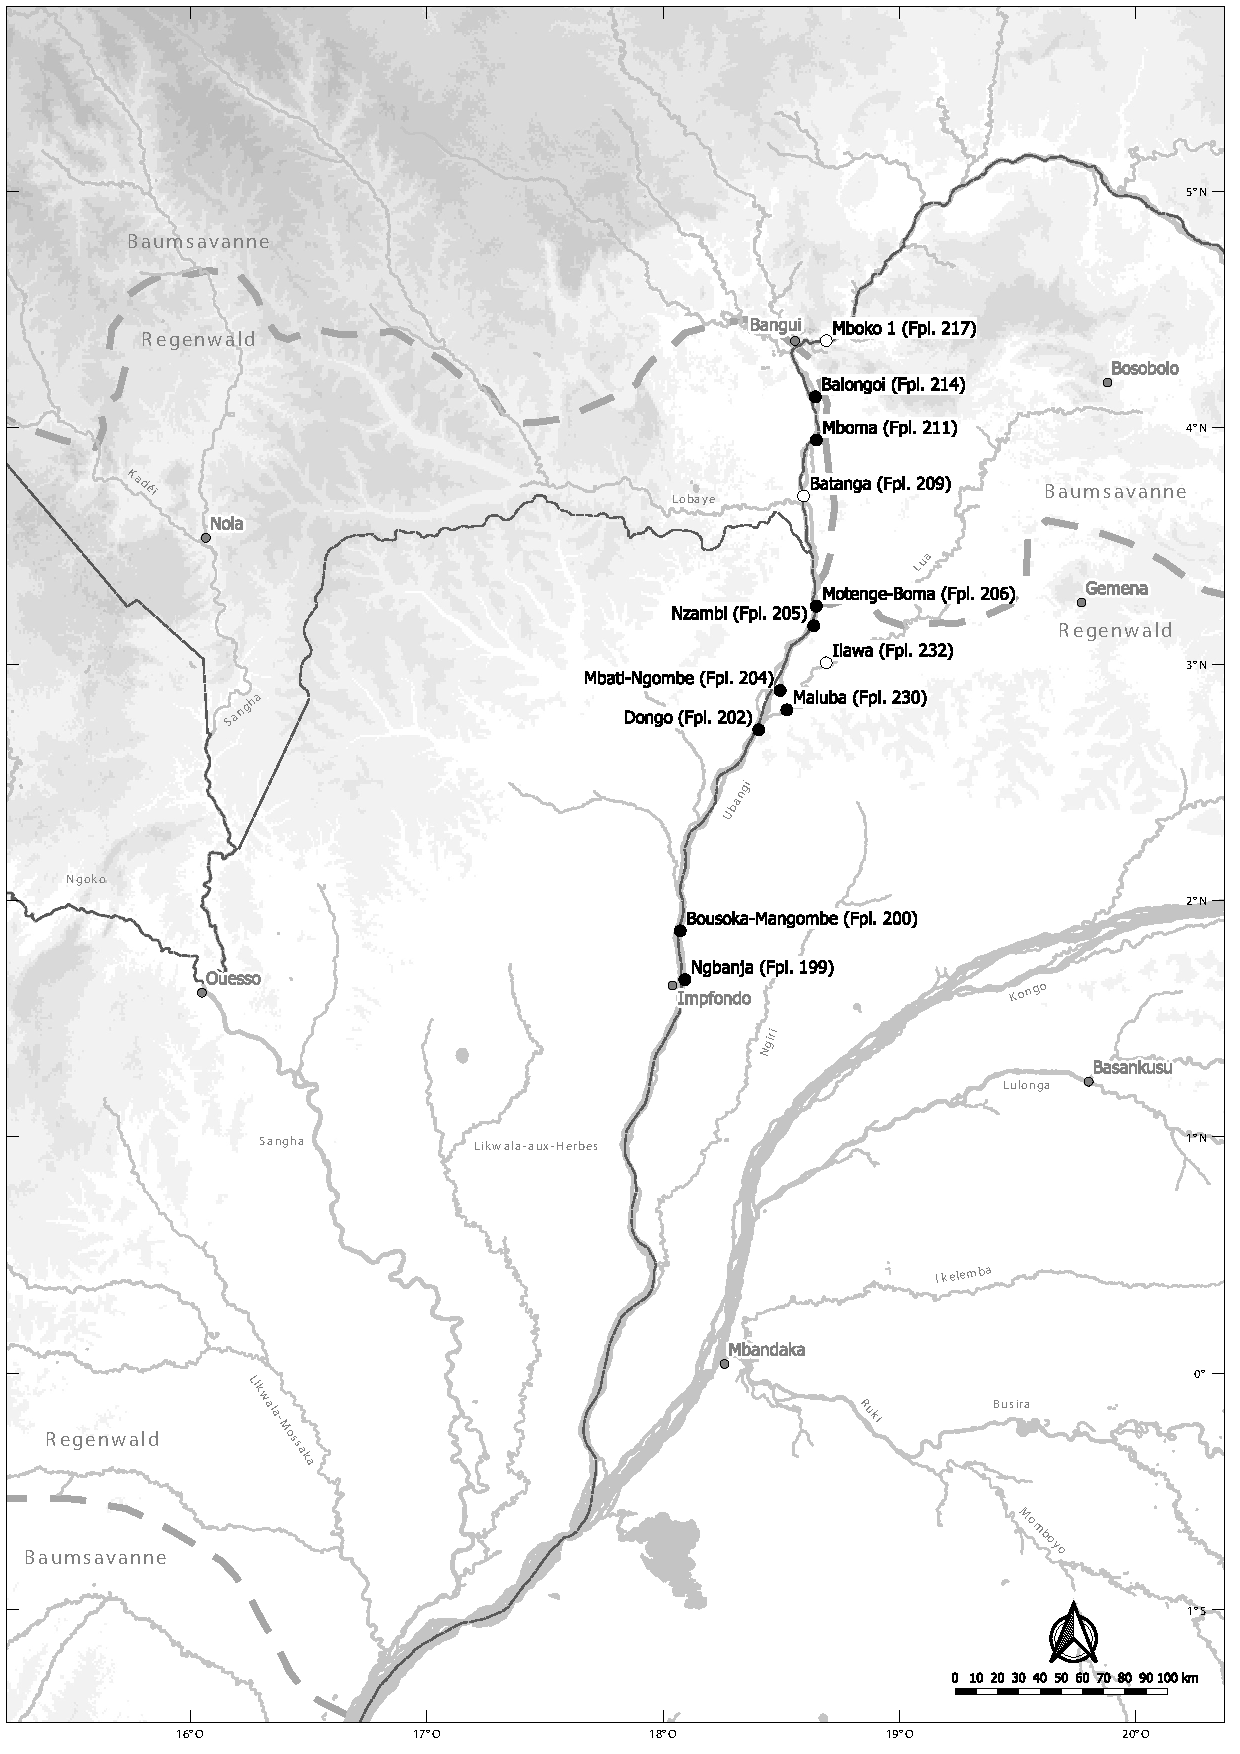
\includegraphics[width=\textwidth]{fig/DON_Verbreitung.pdf}
	\caption{Dongo-Gruppe: Verbreitung.}
	\label{fig:DON_Verbreitung}
\end{figure*}

\paragraph{Datierung}\hspace{-.5em}|\hspace{.5em}%
Für die Keramik der Dongo-Gruppe liegen keine absoluten Daten vor. Eine chronologische Einordnung der beschriebenen und zu einer Stilgruppe zusammengefassten Formen lässt sich daher nur anhand relativ-chronologischer Indizien, im Vergleich mit anderen Stilgruppen des Arbeitsgebietes erzielen. Eine dieser Ähnlichkeiten ergibt sich zu den Stilen Batalimo-Maluba (Kap.~\ref{sec:BTM-Gr}) und \mbox{Ngbanja} (Kap.~\ref{sec:NGB-Gr}), die wie auch die Dongo-Keramik innenseitig mit feinen Rillenbündeln versehene Ränder aufweisen (Abb.~\ref{Fig-BatMLB-Typvertreter}.5, \ref{fig:NGB_Typverteter}.6). Die umgelegten Ränder der Dongo-Gruppe (Abb.~\ref{fig:DON_Typverteter}.1, 9) zeigen hingegen bedingte Ähnlichkeiten zur Randgestaltung des Motenge-Boma-Stils (Kap.~\ref{sec:MTB-Gr}; Abb.~\ref{fig:MTB_Typvertreter}.4, 6--7, 9). Auch die sehr seltene Rouletteverzierung weist auf einen Bezug der Dongo-Keramik zu jüngeren Stilgruppen entlang des \mbox{Ubangi}, wie Mokelo (Kap.~\ref{sec:MKL-Gr}), Motenge-Boma (Kap.~\ref{sec:MTB-Gr}), Dama (Kap.~\ref{sec:DAM-Gr}) oder Mbati-Ngombe (Kap.~\ref{sec:MBN-Gr}) hin. Die im Grundsatz eher spärliche Verzierungspraxis innerhalb der Dongo-Keramik findet ihre Entsprechung in der ebenfalls nur wenig verzierten Keramik der Bobulu-Gruppe (Kap.~\ref{sec:BBL-Gr}). Vor dem gegenwärtigen Quellenstand kann der Dongo-Keramik nur grob eine chronologische Stellung zwischen den ältesten keramischen Formen des Arbeitsgebietes, den Gruppen Batalimo-Maluba und \mbox{Ngbanja}, sowie den jüngeren und jüngsten Gruppen Mokelo, Motenge-Boma, Dama sowie Mbati-Ngombe eingeräumt werden. Auf Basis der vorliegenden Datierungsansätze wird für die Dongo-Keramik eine provisorische Alterspanne zwischen dem 9./10. und 15./16.~Jh. n.~Chr. angenommen.


\paragraph{Verbreitung}\hspace{-.5em}|\hspace{.5em}%
Die der Dongo-Gruppe zugewiesene Keramik fand sich in zwölf Fundstellen, vor allem entlang des mittleren \mbox{Ubangi} (Abb.~\ref{fig:DON_Verbreitung}). Die südlichste Fundstelle, die sicher Keramik der Dongo-Gruppe erbrachte, ist \mbox{Ngbanja} (Fpl.~199). Im Norden fanden sich sichere Dongo-Funde bis nach Balongoi (Fpl.~214), direkt stromab des \mbox{Ubangi}-Bogens. Ein weiterer, möglicher Vertreter dieses Stils fand sich etwas weiter nördlich in Mboko~I (Fpl.~217). Daneben wurden in Ilawa am Lua (Fpl.~232) zwei potenzielle Vertreter der Dongo-Gruppe erfasst. Bis auf das eingangs genannte Stück aus Maluba am Lua (Fpl.~230) wurde keine Dongo-Keramik in einem ausgegrabenen Kontext gefunden, da aber die einzigen Grabungen im Bereich der Flüsse \mbox{Ubangi} und Lua in Maluba durchgeführt wurden (Kat.-Nr.~1--5), verwundert dies nicht weiter. In Anbetracht dieses Umstandes muss die Keramik der Dongo-Gruppe als reiner Komplex aus Survey-Funden charakterisiert werden und entzieht sich damit einer zweifelsfreien chronologischen Ansprache.
